%%%%%%%%%%%%%%%%%%%%%%%%%%%%%%%%%%%%%%%%%%%%%%%%%
\documentclass[11pt,letterpaper]{report}

%##################################################################################################

\usepackage{color}
    \definecolor{dark_blue}{rgb}{0,0,0.6}
    \definecolor{light_blue}{rgb}{0,0.4,0.8}
    \definecolor{dark_vilet}{rgb}{0.4,0,0.4}
\usepackage{fancybox}
\usepackage{wallpaper}
\usepackage{url}
\usepackage[colorlinks,
            linkcolor=dark_vilet,
            citecolor=light_blue,
            urlcolor=dark_blue]{hyperref}
\usepackage{colortbl}
\usepackage{amssymb}
\usepackage{amsmath}
\usepackage{graphicx}
\usepackage{algorithm}
\usepackage{algorithmic}
%\usepackage[square,comma,sort&compress]{natbib}
\usepackage[Sonny]{fncychap}
%%\usepackage{fancyhdr}
\usepackage{titletoc}
\usepackage[scaled=.92]{helvet}
\usepackage{mathptmx}
\usepackage{subfigure}
\usepackage{xspace}
\usepackage{multirow}

%\renewcommand{\headrulewidth}{0.5pt}
%\renewcommand{\footrulewidth}{0.5pt}
\ChTitleVar{\huge\sf}
\ChNameVar{\Huge\sf}
%\rhead{}

\newcommand{\cdl}[1]{\textsf{#1}}
\newenvironment{link_url}
{\begin{description}
    \item}
{\end{description}}
\newenvironment{cmd_line}
{\begin{description}
    \item}
{\end{description}}

\newcommand{\ignore}[1]{}
\newcommand{\tabwidth}[0]{.45\linewidth}
\newcommand{\figwidth}[0]{.48\linewidth}

\newcommand\prjfnt{{\small \fontfamily{pag}\selectfont{}}\xspace}
\newcommand\gefnt{{\small \fontfamily{ppl}\selectfont{}}\xspace}
\newcommand{\PLASMA}{{\prjfnt{PLASMA}}\xspace}
\newcommand{\MAGMA}{{\prjfnt{MAGMA}}\xspace}
\newcommand{\TBLAS}{{\prjfnt{TBLAS}}\xspace}
\newcommand{\PBLAS}{{\prjfnt{PBLAS}}\xspace}
\newcommand{\PESSL}{{\prjfnt{PESSL}}\xspace}
\newcommand{\ESSL}{{\prjfnt{ESSL}}\xspace}
\newcommand{\SMPSS}{{\prjfnt{SMPSs}}\xspace}
\newcommand{\SMPSs}{{\prjfnt{SMPSs}}\xspace}
\newcommand{\MKL}{{\prjfnt{MKL}}\xspace}
\newcommand{\SCALAPACK}{{\prjfnt{ScaLAPACK}}\xspace}
\newcommand{\LAPACK}{{\prjfnt{LAPACK}}\xspace}
\newcommand{\LINPACK}{{\prjfnt{LINPACK}}\xspace}
\newcommand{\EISPACK}{{\prjfnt{EISPACK}}\xspace}
\newcommand{\DPOTRF}{{\gefnt{DPOTRF}}\xspace}
\newcommand{\DGEQRF}{{\gefnt{DGEQRF}}\xspace}
\newcommand{\DGETRF}{{\gefnt{DGETRF}}\xspace}
\newcommand{\DGEMM}{{\gefnt{DGEMM}}\xspace}
\newcommand{\BLAS}{{\gefnt{BLAS}}\xspace}
\newcommand{\BLACS}{{\gefnt{BLACS}}\xspace}
\newcommand{\dgemm}{{\gefnt{dgemm-seq}}\xspace}
\newcommand{\dssrfb}{{\gefnt{dssrfb-seq}}\xspace}
\newcommand{\dssssm}{{\gefnt{dssssm-seq}}\xspace}
\newcommand{\Intel}{{\gefnt{Intel64}}\xspace}
\newcommand{\Power}{{\gefnt{Power6}}\xspace}

%##################################################################################################


%%\usepackage{framed}
\usepackage[margin=1.0in]{geometry}
\usepackage{url}
\usepackage{alltt}
\usepackage{listings}
\lstset{ %
  basicstyle=\scriptsize,               % the size of the fonts that are used for the code
  %numbers=left,                   % where to put the line-numbers
  %numberstyle=\footnotesize,      % the size of the fonts that are used for the line-numbers
  %stepnumber=2,                   % the step between two line-numbers. If it's 1, each line
  %numbersep=5pt,                  % how far the line-numbers are from the code
  %backgroundcolor=\color{white},  % choose the background color. You must add \usepackage{color}
  %showspaces=false,               % show spaces adding particular underscores
  %showstringspaces=false,         % underline spaces within strings
  %showtabs=false,                 % show tabs within strings adding particular underscores
  frame=lines,                   % adds a frame around the code lines single
  %tabsize=2,                      % sets default tabsize to 2 spaces
  %captionpos=b,                   % sets the caption-position to bottom
  %breaklines=true,                % sets automatic line breaking
  %breakatwhitespace=false,        % sets if automatic breaks should only happen at whitespace
  %title=\lstname,                 % show the filename of files included with \lstinputlisting;
  % also try caption instead of title
  %escapeinside={\%*}{*)},         % if you want to add a comment within your code
  %morekeywords={*,...}            % if you want to add more keywords to the set
  language=C
}


\begin{document}

%%%%%%%%%%%%%%%%%%%%%%%%%%%%%%%%%%%%%%%%%%%%%%%%%%%

\thispagestyle{empty}
\begin{flushright}
\sf
\noindent
{\Huge\textbf{QUARK Users' Guide}}
\rule[-1ex]{\textwidth}{5pt}\\[2.5ex]
{\Large\textbf{QUeueing And Runtime for Kernels}} \\
\vspace{0.1in}
{\Large{Version: April 2011}} \\ %% FIXME
\vspace{0.5in}
\noindent
Electrical Engineering and Computer Science \\
Innovative Computing Laboratory \\
\textbf{University of Tennessee}

%% \vspace{1.1in}
%% {\Large\textbf{DRAFT: PLEASE DO NOT REDISTRIBUTE}} \\
%% This report is still being updated.\\
%% A final version will be available soon.\\

\vspace{2.0in}
\noindent
Asim YarKhan \\
Jakub Kurzak \\
Jack Dongarra \\
\end{flushright}

%%%%%%%%%%%%%%%%%%%%%%%%%%%%%%%%%%%%%%%%%%%%%%%%%%%

\tableofcontents
%%\pagenumbering{roman}
%%\pagestyle{fancy}
\setlength\parindent{0in}
\setlength\parskip{0.1in}
\sloppy
\rm


%%%%%%%%%%%%%%%%%%%%%%%%%%%%%%%%%%%%%%%%%%%%%%%%%%%

%% \pagebreak
%% {\LARGE {NOTES and TODO} }
%% \begin{itemize}
%% \item Installing QUARK - Do we need this at present?  Can it even be
%%   done? Given that QUARK is not separate download from PLASMA.
%%   \begin{itemize}
%%   \item List tested platform and compilers
%%   \item Prerequisites - pthreads or windows threads
%%   \item Optional HWLOC - perhaps describe default core binding
%%     process, since it can be awkward on a multi-user shared
%%     environment.  Also, how to prevent core binding if needed.
%%   \item Optional Eztrace - Mathieu included optional eztrace stuff for
%%     PLASMA usage, but I am not sure how much that depends on PLASMA.
%%     I will not mention it at present.  Normally it should not be
%%     enabled.
%%   \item Windows status - I think that this would be part of a
%%     installation guide and would describe the Cmake build process on
%%     windows.
%%   \end{itemize}
%% \item Suitability - For what kinds of problems is QUARK suitable?  For
%%   example, it does not support recursive task insertion (task inserts
%%   more tasks).
%% \item Data hazard avoidance - This is fragile and it is disabled by
%%   default.  Skipping it.
%% \item Side note:  There is a lot of inconsistency in the API, though
%%   it is probably a bit late for this!
%%   \begin{itemize}
%%   \item Quark *quark; Maybe that should be QUARK *quark;
%%   \item quark\_unpack\_args\_2: These macros should be
%%     QUARK\_Unpack\_Args\_2
%%   \item Sometimes it is QUARK\_Task\_Flag\_Set (QUARK\_thing\_action)
%%     and sometimes it is QUARK\_Get\_Task\_Label (QUARK\_action\_thing)
%%     - Mostly it is QUARK\_action\_thing, and all the calls should
%%     follow that convention.
%%   \item QUARK\_Waitall + QUARK\_Free versus QUARK\_Delete - the names
%%     are not self evident
%%   \item QUARK\_Setup versus QUARK\_New: Names are not self evident.
%%   \end{itemize}
%% \end{itemize}
%% \pagebreak

%%%%%%%%%%%%%%%%%%%%%%%%%%%%%%%%%%%%%%%%%%%%%%%%%%%

%%\input{introduction}
\chapter{Introduction}

QUARK (QUeueing And Runtime for Kernels) is a runtime environment for
the dynamic scheduling and execution of applications that consist of
precedence-constrained kernels on multicore, \mbox{multi-socket}
shared memory systems.  The goal of the project is to provide an
easy-to-use interface to application programming, with an efficient
implementation which will scale to large shared memory architectures.
The main design principle behind QUARK is implementation of the
dataflow model, where scheduling is based on data dependencies between
tasks in a task graph.  The data dependencies are inferred through a
runtime analysis of data hazards implicit in the data usage by the
kernels.

The focus of QUARK development is to support dynamic linear algebra
algorithms for the \PLASMA linear algebra project
\cite{Agullo:2010:PLASMA-Users}.  However, QUARK is capable of
supporting other application domains where the application can be
decomposed into tasks with data dependencies.

%% QUARK should run on architectures ...FIXME

\section{Overview of QUARK}

Given a serial code composed of calls to kernel routines acting on
contiguous data, QUARK can be used to allow the kernel routines to
execute asynchronously in parallel on a shared memory architecture.
The serial nature of the original code is preserved by enforcing the
data dependencies between the kernels.  In order to support this, the
kernel calls need to be extended to express the data sizes and the I/O
usage.  For example, for kernel routine $function_K$, parameter $A$ is
specified to be $2000$ bytes long and is used as \verb|INOUT| by this
kernel.  QUARK uses the parameter specifications to infer the
dependencies between the various kernel routines in the application.
  These dependencies form an implicit DAG (Directed Acyclic Graph)
 connecting the kernel routines.
\begin{figure}[bt]
  \centering 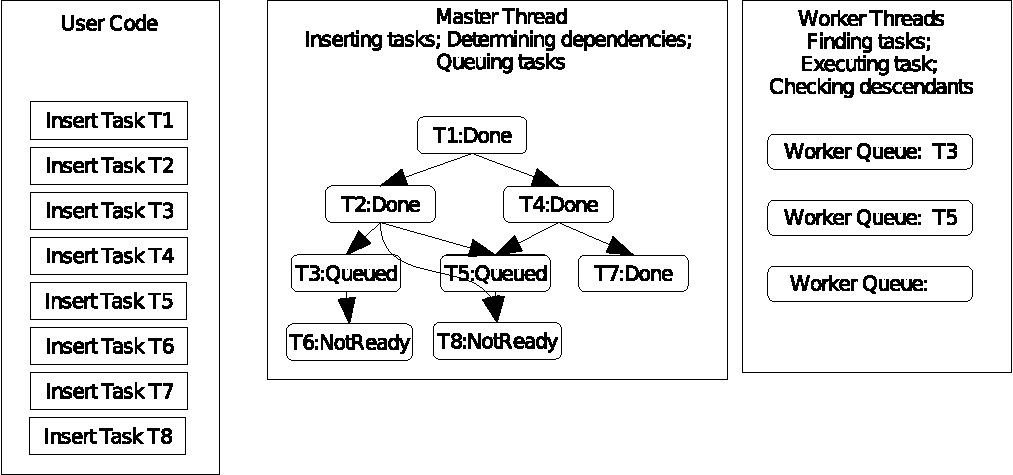
\includegraphics[trim=0 0 0 0, clip,
    width=1.0\columnwidth]{scheduler_architecture}
  \caption{Idealized architecture diagram for the QUARK shared-memory
    runtime environment.  Users thread runs serial code and acting as
    the master inserts tasks into a (implicit) DAG based on their
    dependencies.  Tasks can be in NotReady, Queued or Done states.
    When dependencies are satisfied, tasks are queued and executed by
    worker threads.  Workers update dependencies when tasks are done.}
  \label{fig:scheduler-architecture}
\end{figure}
Fig.~\ref{fig:scheduler-architecture} provides an idealized overview
of the architecture of the QUARK runtime environment.

Please note, in this document, the terms function, kernel and task may
be used interchangeably to refer to a function that is to be executed
by the QUARK runtime system.  Additionally, depending on the context,
the terms argument, parameter or data item may all be used to refer to
the parameters of a function.


\subsection{Performance Goals}

Since the development of QUARK is driven by the needs of the PLASMA
linear algebra library, it needs to meet very high goals with respect
to performance.  A substantial portion of the PLASMA library can be
executed using a static scheduler as well as the dynamic QUARK
execution environment, and the performance of QUARK needs to be
comparable to that of the static scheduler.  Given that the static
scheduler has no overheads, QUARK cannot exceed its performance on
basic algorithms.  However, the use of QUARK enables some
optimizations (e.g., DAG merging, loop reordering, discussed later)
that cannot be done by the static scheduler.  Additionally, preparing
a static execution schedule for complex algorithms is a very
substantial challenge.  Programming using the QUARK API is much easier
for most developers to use, and it allows developers to experiment
with alternative algorithmic formulations.

\subsection{Related Projects}

The ubiquity of multi-core processors in current hardware has led to
the emergence of a myriad of multithreading frameworks embracing the
idea of task scheduling: Cilk \cite{Blumofe:1995:Cilk:-an-efficient},
OpenMP (tasking features)~\cite{:2008:OpenMP-Application}, Intel
Threading Building Blocks~\cite{Reinders:2007:Intel-threading}, just
to name a few prominent examples.  One especially relevant category
are multithreading systems based on {dataflow} principles, which
represent the computation as a {\em Direct Acyclic Graph}~(DAG) and
schedule tasks at runtime through resolution of data hazards. The
QUARK project falls within this category. Two similar academic
projects are SMPSs~\cite{Perez:2008:A-dependency-aware-task-based}
from Barcelona Supercomputer Center and
StarPU~\cite{Augonnet:2009:StarPU:-A-Unified} from INRIA Bordeaux.
While these three systems have their strengths and weaknesses, QUARK
has vital extensions for use in a numerical library.


\subsection{License Information}

QUARK is a software package provided by University of Tennessee.
QUARK's license is a BSD-style permissive free software license
(properly called modified BSD).  It allows proprietary commercial use,
and for the software released under the license to be incorporated
into proprietary commercial products.  Works based on the material may
be released under a proprietary license as long as QUARK's license
requirements are maintained, as stated in the LICENSE file, located in
the main directory of the QUARK distribution.  In contrast to copyleft
licenses, like the GNU General Public License, QUARK's license allows
for copies and derivatives of the source code to be made available on
terms more restrictive than those of the original license.


%%%%%%%%%%%%%%%%%%%%%%%%%%%%%%%%%%%%%%%%%%%%%%%%%%%

\chapter{Basic Usage of the QUARK API}

QUARK is often used as a library for a serial application, where QUARK
does all the thread and resource management.  There is an alternate
mode where QUARK does not do internal thread management so it can be
used as part of a multi-threaded library; this is described later.

\begin{figure}[bp]
\centering
\begin{lstlisting}
    #include "quark.h"
    
    /* This task unpacks and prints a string.  At each call, the idx
       character  is replaced with an underscore, changing the string. */
    void hello_world_task( Quark *quark ) {
      int idx; char *str;
      quark_unpack_args_2( quark, idx, str );
      printf( "%s\n", str );
      str[idx] = '_';
    }
    
    /* A simple variation of "Hello World" */
    main() {
      int idx;
      char str[] = "Hello World";
      Quark *quark = QUARK_New( 2 );
      for ( idx=0; idx<strlen(str); idx++ )
          QUARK_Insert_Task( quark, hello_world_task, NULL,
              sizeof(int), &idx, VALUE,
              strlen(str)*sizeof(char), str, INOUT,
              0 );
      QUARK_Delete( quark );
    }
\end{lstlisting}
\caption{Basic QUARK program, showing the setup of QUARK, task
  insertion with simple dependency information, and shutdown of
  QUARK. }
\label{fig:quark_basic_example}
\end{figure}

\section{Hello World}  
Fig.~\ref{fig:quark_basic_example} shows a
variation of ``Hello World'' which demonstrates many of the basic
features of QUARK.  This is a fully functional C program that
demonstrates how a simple program in QUARK may be implemented.

First, a new QUARK instance is created in the main program with two
threads, the master and one spawned worker thread.  Then, at each
iteration of the loop in the main program, a new is inserted into the
QUARK runtime system.  The task will call the function
\verb|hello_world_task| when it is executed by the runtime.  The
\verb|idx| argument is passed as \verb|VALUE| parameter, since is
unchanged by the function.  The \verb|str| argument is marked
\verb|INOUT| since the string will be altered by the
\verb|hello_world_task|.  In this simple program, the use of a
\verb|INOUT| dependency keeps the serialized semantics of the original
loop.

In \verb|hello_world_task|, the data is unpacked from QUARK and
assigned to the \verb|idx| and \verb|str| variables using the unpack
macro.  The string is then printed, and after that it is altered by
changing the \verb|idx| character to an underscore.  This allows us to
see how the string is changed by each task, and to note that the
original serial order of the code is being preserved by multiple tasks
running on multiple threads.  The output of this program is shown in
Fig.~\ref{fig:quark_basic_example_output}
\begin{figure}[bp]
\centering
\begin{lstlisting}
    Hello World
    _ello World
    __llo World
    ___lo World
    ____o World
    _____ World
    ______World
    _______orld
    ________rld
    _________ld
    __________d
\end{lstlisting}
\caption{Output from the Basic QUARK program in Fig.~\ref{fig:quark_basic_example}. }
\label{fig:quark_basic_example_output}
\end{figure}

More details of the various QUARK calls involved in this code are
given here.
\paragraph{Initializing QUARK}
The \verb|QUARK_New| call initializes the library, and spawns and
manages \verb|num_threads| threads (including the master) to handle
the computation.  If \verb|num_threads < 1|, QUARK will first check
the \verb|QUARK_NUM_THREADS| environment variable, then use as many
threads as there are cores.
\pagebreak[3]
\begin{samepage}
\begin{lstlisting}
    Quark *QUARK_New(int num_threads);
\end{lstlisting}
\end{samepage}
\pagebreak[3]

\paragraph{Adding tasks}
After initializing, tasks can be added to the QUARK runtime system by
the master thread.  The \verb|QUARK_Insert_Task| call has many options,
however only the basic usage is shown here.
\begin{samepage}
\begin{lstlisting}
QUARK_Insert_Task( Quark *quark, void (*function) (Quark *),
    Quark_Task_Flags *tflags,
    int sizeof_arg_1_in_bytes, void *arg_1, int arg_1_flags,
    int sizeof_arg_2_in_bytes, void *arg_2, int arg_2_flags,
    ...,
    0 );
\end{lstlisting}
\end{samepage}
The first two parameters are the QUARK data structure and a pointer to
the function that is to be executed.  The task flags \verb|tflags| can
be used to provide tasks specific information, such as the priority of
the task or a sequence tag used to group related tasks.  For basic
usage, the tasks flags can be set to NULL.  More advanced usage of the
task flags will be described later.

The argument parameters to given to the \verb|function| are passed as
\verb|varargs|.  Each argument is presented as a triplet: the size of
the argument in bytes, a pointer to the argument, and a flag
indicating the way that the argument is to be used.  This sequence of
triplets is terminated by sending a 0 as the argument size.  The
argument flag can be one of \verb|VALUE|, \verb|INPUT|, \verb|OUTPUT|,
\verb|INOUT|, \verb|NODEP| and \verb|SCRATCH|.  These denote different
ways that the argument is going to be used by \verb|function|.  Here,
we describe the meaning of \verb|VALUE| and \verb|INOUT|.  The other
argument flags will be described later in this guide.
\begin{description}
\item[]\verb|VALUE| The parameter data is copied to the QUARK task and
  is not used for dependency resolution.  Since the parameter is
  copied over, it can be altered by the master thread without
  affecting the task.
\item[]\verb|INOUT| The parameter is used as input as well as output
  in the \verb|function|.  Preceding reads and writes must be
  satisfied before this \verb|function| can be executed.
\end{description}
QUARK schedules the \verb|function| for execution when all the
dependencies for the data arguments (\verb|arg_1|, \verb|arg_2|, ...)
are satisfied.

\paragraph{Finalizing QUARK}
When the user is done with inserting all their tasks, they will need to
call \verb|QUARK_Delete| to wait for the QUARK runtime to finish
executing any remaining tasks and release the QUARK data structures.
All the spawned worker threads will also be finalized by this call.
\begin{samepage}
\begin{lstlisting}
void QUARK_Delete(Quark * quark);
\end{lstlisting}
\end{samepage}

%% The following shows how a BLAS matrix multiplication wrapper function
%% \verb|SCHED_dgemm| would be inserted with all the standard arguments
%% for \verb|dgemm| matrix multiplication.
%% \begin{lstlisting}
%% QUARK_Insert_Task( quark, SCHED_dgemm, NULL,
%%     sizeof(char),         "N",        VALUE,
%%     sizeof(char),         "T",        VALUE,
%%     sizeof(int),          &m,         VALUE,
%%     sizeof(int),          &n,         VALUE,
%%     sizeof(int),          &k,         VALUE,
%%     sizeof(double),       &alpha,     VALUE,
%%     sizeof(double)*NB*NB, A,          INPUT,
%%     sizeof(int),          &lda,       VALUE,
%%     sizeof(double)*NB*NB, B,          INPUT,
%%     sizeof(int),          &ldb,       VALUE,
%%     sizeof(double),       &beta,      VALUE,
%%     sizeof(double)*NB*NB, C,          INOUT,
%%     sizeof(int),          &ldc,       VALUE,
%%     0 );
%% \end{lstlisting}
%% The QUARK runtime will store the arguments, and when all the data
%% dependencies (\verb|INPUT|, \verb|INOUT|, \verb|OUTPUT|) are
%% satisfied, QUARK will schedule \verb|SCHED_dgemm| for execution by a
%% worker thread.

%% The wrapper function \verb|SCHED_dgemm| function will need to unpack
%% the arguments to retrieve them from QUARK.  Then the wrapper makes a
%% call to a Fortran matrix multiplication routine \verb|dgemm|.
%% \begin{lstlisting}
%% void SCHED_dgemm(Quark *quark) {
%%     char transa; char transb;
%%     int m; int n; int k;
%%     double alpha; double *A; int lda;
%%     double *B; int ldb;
%%     double beta; double *C; int ldc;
%%     quark_unpack_args_13(quark, transa, transb, m, n, k,
%%         alpha, A, lda, B, ldb, beta, C, ldc);
%%     dgemm_(&transa, &transb, &m, &n, &k, &alpha, A,
%%         &lda, B, &ldb, &beta, C, &ldc);
%% }
%% \end{lstlisting}



%%%%%%%%%%%%%%%%%%%%%%%%%%%%%%%%%%%%%%%%%%%%%%%%%%%

\chapter{Advanced Usage}

QUARK offers a number of features that allow finer control over the
runtime system and the task scheduling and execution.  Most these
features are controlled either via the task flags passed into each
task, or via the argument flags provided to the various arguments.  A
few global features are enabled using environment variables.  The
features are described and summarized here.

\paragraph{Task Scheduling}
In order to make sense of some of the features, the default task
scheduling method in QUARK needs to be outlined.  At a very high
level, QUARK uses data locality information to assign tasks whose
dependencies are satisfied to threads where there may be data reuse.
The threads execute assigned tasks using a FIFO priority queue.  A
thread that does not have any assigned tasks may steal tasks from the
back of the queue of another thread using LIFO work-stealing policy.

\paragraph{Data Locality}
QUARK will attempt to use data locality information in making
decisions about where to schedule tasks.  In the current version of
QUARK, the arguments will be examined to determine the output data.
The task will be assigned by default to the same thread that has
previously written that output data.  This heuristic should enable
cache reuse under many practical circumstances.


\section{Argument Flags}

When a task is inserted into the QUARK runtime system, its parameters
are specified as triplets.  The parameter size in bytes, a pointer to
the parameter (even scalers need to be passed by reference), and some
flags that are used to specify how the parameter is going to be used by
the task and how dependencies on that parameter are to be resolved.
The parameter must always specify its usage as one of the following:
\verb|VALUE|, \verb|INPUT|, \verb|OUTPUT|, \verb|INOUT|, \verb|NODEP|
and \verb|SCRATCH|.
\begin{samepage}
\begin{lstlisting}
QUARK_Insert_Task( Quark *quark, void (*function) (Quark *),
    int sizeof_arg_1_in_bytes, void *arg_1, int arg_1_flags,
    int sizeof_arg_2_in_bytes, void *arg_2, int arg_2_flags,
    ...,
    0 );
\end{lstlisting}
\end{samepage}
\begin{description}
\item[]\verb|VALUE| The parameter data is copied to the QUARK task and
  is not used for dependency resolution.
\item[]\verb|INPUT| The parameter is used as input only in the
  \verb|function|; preceding write operations on this data must be
  satisfied before this \verb|function| can be executed.
\item[]\verb|INOUT| The parameter is used as input as well as output
  in the \verb|function|.  Preceding reads and writes must be
  satisfied before this \verb|function| can be executed.
\item[]\verb|OUTPUT| This parameter is used as output.  Preceding
  reads and writes must be satisfied before this \verb|function| can
  be executed.
\item[]\verb|NODEP| The parameter is declared by the programmer to not
  cause any dependency.  This allows a programmer flexibility in
  forcing scheduling; however it should be used with caution.
  Sometimes this is used if the programmer knows that sufficient
  dependencies are maintained by other parameters.
\item[]\verb|SCRATCH| The parameter is declared as temporary scratch
  space, and if the parameter pointer is NULL, QUARK will allocate the
  data when needed and pass it to \verb|function|.
\end{description}

In addition, for parameters that may involve dependencies (i.e.,
\verb|INPUT|, \verb|INOUT|, \verb|OUTPUT|) some optional information
can be passed in via the parameter flags.
\begin{description}
\item[]\verb|ACCUMULATOR| A parameter that is flagged as ACCUMULATOR
  and accessed successively by a set of tasks is accumulating data
  within that parameter.  This lets QUARK know that the access to this
  parameter by those tasks can be safely reordered.
\item[]\verb|GATHERV| This flag declares to QUARK that the data is
  being gathered into the data parameter in a non-conflicting manner.
  A successive series of \verb|GATHERV| accesses to this data parameter
  can safely be performed simultaneously.
\item[]\verb|LOCALITY|  This flag lets QUARK know that data locality
  and cache reuse should follow this data item.  If possible, multiple
  tasks using this data item should be run on the same thread.
\item[]\verb|QUARK_REGION_X| A parameter can be viewed as consisting
  as the union of eight sub-regions (\verb|QUARK_REGION_0| thru
  \verb|QUARK_REGION_7|).  Using these region flags allows the
  dependency processing to work on subsets of the entire data region.
  If regions are used, they should combine to cover eight sub-regions.
\end{description}
\pagebreak[3]
The following gives some idea of how the various parameter flags may
be combined to provide information to QUARK.
\pagebreak[3]
\begin{samepage}
\begin{lstlisting}
QUARK_Task_Insert( quark, function, &tflags,
    size_of_data, ptr_to_data, arg_flags,
    sizeof(int), &N, VALUE,
    N*N*sizeof(double), ptr_to_A, INOUT | ACCUMULATOR,
    N*N*sizeof(double), B, INOUT | LOCALITY,
    N*N*sizeof(double), C, INPUT | QUARK_REGION_1 | QUARK_REGION_2 | QUARK_REGION_3,
    N*N*sizeof(double), D, INOUT | QUARK_REGION_4,
    N*N*sizeof(double), E, INOUT | QUARK_REGION_5 | QUARK_REGION_6 | QUARK_REGION_7,
    N*N*sizeof(double), F, INOUT | GATHERV,
    ... , 0 )
\end{lstlisting}
\end{samepage}
\pagebreak[3]

\section{Task Flags}

QUARK passes task specific information to the runtime system using
task flags.  These flags can specify things such as a color and label
for visualizing the task DAG, priorities used for scheduling the task,
and a way to collect tasks into sequences for error handling.  Task
flags are created and initialized as shown here; any flag that is not
specified will have a default value.  More information about the usage
of the various flags follows.
\pagebreak[3]
\begin{samepage}
\begin{lstlisting}
    Quark_Task_Flags tflags = Quark_Task_Flags_Initializer;
    QUARK_Task_Flag_Set( &tflags, TASK_COLOR, "red" );
    QUARK_Task_Flag_Set( &tflags, TASK_LABEL, "my_DGEMM" );
    QUARK_Task_Flag_Set( &tflags, TASK_PRIORITY, 100 );
    QUARK_Task_Flag_Set( &tflags, TASK_LOCK_TO_THREAD, thread_number );
    QUARK_Task_Flag_Set( &tflags, TASK_SEQUENCE, sequence_ptr );
    QUARK_Task_Flag_Set( &tflags, TASK_THREAD_COUNT, num );
    QUARK_Task_Flag_Set( &tflags, TASK_SET_TO_MANUAL_SCHEDULING, 0_or_1 );
    QUARK_Task_Insert( quark, function, &tflags, ... , 0 )
    // Task flags for the current task can be obtained using
    intptr val = QUARK_Task_Flag_Get( quark, \textit{TASK_FLAG_NAME} );
\end{lstlisting}
\end{samepage}
\pagebreak[3]

\subsection{Visualizing Runtime DAGs}
QUARK can generate GraphViz \cite{Ellson:2002:Graphviz-Open} files at
runtime that represent the DAG of executed tasks.  To enable this
feature, set the environment variable \verb|QUARK_DOT_DAG_ENABLE=1|.
By default, the graph will have no labels on nodes and all nodes have
the same color.  It is possible to change the display of the DAG nodes
by setting task flags when the \verb|QUARK_Insert_Task| function is
called.  The color strings that can be used are described in the
GraphViz documentation.
\begin{samepage}
\begin{lstlisting}
    Quark_Task_Flags tflags = Quark_Task_Flags_Initializer;
    QUARK_Task_Flag_Set( &tflags, TASK_COLOR, "red" );
    QUARK_Task_Flag_Set( &tflags, TASK_LABEL, "my_DGEMM" );
    QUARK_Task_Insert( quark, function, &tflags, ... , 0 )
\end{lstlisting}
\end{samepage}
After the program executes. the DAG will be written to file in the
execution directory with the name ``\verb|dot_dag_file.dot|''.  Please
see the GraphViz documentation on how to manipulate this file.  For
example, to setup DAG generation, execute, and translate the generated
DAG to a PDF format use the following commands.
\begin{samepage}
\begin{lstlisting}
    export QUARK_DOT_DAG_ENABLE=1
    ./execute_my_quark_binary
    dot -Tpdf -o mydag.pdf dot_dag_file.dot
\end{lstlisting}
\end{samepage}
Standard dependencies between tasks are shown as black arrows, red
arrows represent Write-After-Read (WAR) dependencies that could be
eliminated by making data copies, green arrows mark parallel task
execution allowed by special \verb|GATHERV| data dependencies
specified by the developer.


\subsection{Assigning Priorities to Tasks}
If the developer has knowledge of the algorithm that specifies some
tasks should have higher priority than other tasks, that information
can be provided to the QUARK runtime environment.  After the
dependencies for various tasks are satisfied, the tasks are assigned
to worker priority-queues.  At that point, higher priority tasks get
executed earlier, which may lead to a execution path that more closely
matches the critical path of the DAG.  The priority value can be any
integer, with the default being priority 0.
\begin{samepage}
\begin{lstlisting}
    Quark_Task_Flags tflags = Quark_Task_Flags_Initializer;
    QUARK_Task_Flag_Set( &tflags, TASK_PRIORITY, 100 );
    QUARK_Task_Insert( quark, function, &tflags, ... , 0 )
\end{lstlisting}
\end{samepage}

\subsection{Task Sequences and Error Handling}
Linear algebra programs can be composed of multiple algorithmic
sequences which can fail or succeed independently.  In order to handle
this requirement, the QUARK dynamic runtime system provides a way to
manipulate sequences of tasks.  If an error situation is detected
during the execution of one algorithm, then the associated sequence
can be canceled, without affecting other parts of the program.  If a task
is added to a sequence that has been canceled, it is silently
skipped.
\begin{samepage}
\begin{lstlisting}
    Quark_Sequence *seq = QUARK_Sequence_Create( quark );
    Quark_Task_Flags tflags = Quark_Task_Flags_Initializer;
    QUARK_Task_Flag_Set( &tflags, TASK_SEQUENCE, seq );
    QUARK_Task_Insert( quark, function, &tflags, ... , 0 )
    // If an error occurs, a task can call
    Quark_Sequence *seq = QUARK_Task_Flag_Get( quark, TASK_SEQUENCE )
    QUARK_Sequence_Cancel( quark, seq );
\end{lstlisting}
\end{samepage}

\subsection{Multi-threaded Tasks}
Under certain circumstances it can be beneficial to assign multiple
threads to a single task.  One example of this is in the panel
factorization step of LU factorization.  Since this task deals with
the entire panel, it can become a bottleneck for the execution unless
multiple threads are assigned to it.  QUARK will call the task
multiple times using multiple threads, however, the management of
these multiple threads is left up to the developer.  There is support
to find out the rank of a thread within the set of multiple threads,
so that a developer can take the appropriate action based on the rank.
Note, multi-threaded tasks are locked to their pre-assigned threads
and cannot be stolen and executed by other threads.
\begin{samepage}
\begin{lstlisting}
    Quark_Task_Flags tflags = Quark_Task_Flags_Initializer;
    QUARK_Task_Flag_Set( &tflags, TASK_THREAD_COUNT, 4 );
    QUARK_Task_Insert( quark, function, &tflags, ... , 0 )
    // Within the task, a developer can call
    int rank = QUARK_Get_RankInTask( quark );
\end{lstlisting}
\end{samepage}

\subsection{Locking Tasks to Threads}
For the developer who knows best, it is possible to lock tasks to
threads. This may be done if there is a strong cache benefit of forcing
a certain set of tasks to run on some specific thread (or core).  When
a task is locked to a thread, it cannot be stolen or reassigned to
another thread.
\begin{samepage}
\begin{lstlisting}
    Quark_Task_Flags tflags = Quark_Task_Flags_Initializer;
    QUARK_Task_Flag_Set( &tflags, TASK_LOCK_TO_THREAD, 3 );
    QUARK_Task_Insert( quark, function, &tflags, ... , 0 )
\end{lstlisting}
\end{samepage}


\subsection{Manual Thread Scheduling}
There are occasions when the developer may want to switch the
scheduling mode of a thread from automatic to manual.  For example,
this thread is going to control a GPU and you wish to assign GPU
specific tasks to the thread with full control.  That thread will no
longer take part in automatic task assignment or work stealing.  The
action of switching a thread to manual scheduling is done by assigning
a specific task to the desired thread, and setting the boolean
\verb|THREAD_SET_TO_MANUAL_SCHEDULING| to 1.  When that task executes,
the thread's scheduling mode will be set to manual.
\begin{samepage}
\begin{lstlisting}
    Quark_Task_Flags tflags = Quark_Task_Flags_Initializer;
    // I want thread 2 to control GPUs and nothing else
    QUARK_Task_Flag_Set( &tflags, TASK_LOCK_TO_THREAD, 2 );
    QUARK_Task_Flag_Set( &tflags, THREAD_SET_TO_MANUAL_SCHEDULING, 1 );
    QUARK_Task_Insert( quark, some_special_function, &tflags, ... , 0 )
\end{lstlisting}
\end{samepage}

\section{Environment Variables}

There are some environment variable that affect the behavior of
QUARK.

\paragraph{Task Window Sizes and DAGs}
For many linear algebra algorithms, the number of tasks is on the
order of $N^3$.  This means that even for relatively small
applications, the DAG can be enormous.  Because of this, QUARK uses a
window of active tasks to keep the number of tasks manageable in terms
of memory usage and scheduling overhead.  The task window size is kept
at reasonable defaults, but may be altered via several environment
variable. The task window size per thread can be set by
\verb|QUARK_UNROLL_TASKS_PER_THREAD=500|, or the total task window
size over all threads can be set by \verb|QUARK_UNROLL_TASKS=5000|.  An
interesting usage of this variable for debugging purposes is to use
\verb|QUARK_UNROLL_TASKS=1| to cause a serial execution of the
program, with one task being inserted into QUARK, executing, and then
the next task being inserted.

\paragraph{Generating DAGs for Visualization}
QUARK can generate GraphViz \cite{Ellson:2002:Graphviz-Open} files at
runtime that represent the DAG of executed tasks.  Setting environment
variable \verb|QUARK_DOT_DAG_ENABLE=1| will cause a file
\verb|dot_dag_file.dot| to be created in the execution directory.  It
is possible to change the visualized display of the DAG nodes by
setting task flags when the \verb|QUARK_Insert_Task| function is
called.


\section{Topics Not Covered Elsewhere}

\subsection{Pipelining DAGs}
%% FIXME put in intro? add julien reference
A dynamic scheduler such as QUARK is expected to be slower than a
static scheduler if they are both executing the same single algorithm
because dynamic scheduling has overheads that are not present in the
static scheduler.  However, a dynamic scheduler has advantages in
certain circumstances.  Firstly, if there are several algorithms that
need to be executed in succession, the static scheduler will run them
one after another, synchronizing between the algorithms.  However, a
dynamic scheduler can interleave the tasks from the various
algorithms, scheduling them when their dependencies are satisfied.
This can lead to a faster execution for certain programs and data
sizes~\cite{Agullo:2011:Towards-an-Efficient}.  Secondly, a dynamic
scheduler can perform runtime optimizations, such as reordering
dependencies (e.g. see \verb|ACCUMULATOR| argument flag), effectively
altering the DAG and speeding up execution.

\subsection{Using QUARK within another multi-threaded library}
QUARK was designed to cooperate with other multi-threaded libraries,
so it can use computation threads spawned externally to QUARK.  This
allows the PLASMA library to easily switch between its internal static
scheduling and the dynamic runtime environment offered by QUARK.  If a
developer wants to manage threads outside QUARK, the master thread
needs to call \verb|QUARK_Setup| to setup Quark data structures .
Then each worker thread which the developer has created externally
needs to call \verb|QUARK_Worker_Loop|, after which the worker will
wait for tasks.  The master thread then adds tasks in the normal way,
When the master thread is done adding tasks, it calls
\verb|QUARK_Waitall|.  The worker threads will finish the current
tasks, and return control to the developers program.  When the master
is all done, it can call \verb|QUARK_Free| to free all structures
allocated by \verb|QUARK_Setup|.
\begin{samepage}
\begin{lstlisting}
    // Master thread sets up data structures
    Quark *QUARK_Setup( int num_threads );
    // Worker threads hand control to QUARK temporarily
    void QUARK_Worker_Loop( Quark *quark, int thread_rank );
    // Master tells spawned threads to finish work and return control
    void QUARK_Waitall( Quark * quark );
    // Master frees data structures
    void QUARK_Free( Quark * quark );
\end{lstlisting}
\end{samepage}

\subsection{List API for Task Arguments}
QUARK provides a secondary list-style API for adding arguments to a
function.  This proves useful in the situation that there are a very
large number of dependencies for a function.  For example, a function
to be executed on a GPU may take a large number of data items, and it
would be simpler to provide that data by looping over
indices\cite{Kurzak:2010:An-Implementation-of-the-Tile}.  A second
situation where a list-style API is useful is when the actual number
of dependencies of a function are not known until runtime, so it is
not possible to use the standard varargs based
\verb|QUARK_Insert_Task| method of adding arguments.
\begin{samepage}
\begin{lstlisting}
    // Create a task data structure to hold arguments
    Quark_Task *task = QUARK_Task_Init( quark, function, task_flags )
    // Add (or pack) the arguments into a task data structure
    QUARK_Task_Pack_Arg( quark, task, arg_size, arg_ptr, arg_flags )
    // Insert the packed task data structure into the scheduler for execution
    QUARK_Insert_Task_Packed( quark, task )
\end{lstlisting}
\end{samepage}


%%%%%%%%%%%%%%%%%%%%%%%%%%%%%%%%%%%%%%%%%%%%%%%%%%%

\chapter{Cholesky Factorization Example}

As an example, we present the pseudocode for the tile Cholesky
factorization in Fig.~\ref{fig:tileCholesky} as an algorithm designer
might view it.  This loop-based formulation of code is relatively
straightforward for a designer of linear algebra algorithms, and
allows flexibility in easily experimenting with algorithms.
\begin{figure}[bt]
  \centering
  \scriptsize
  \begin{lstlisting}
    for k = 0..TILES-1
      A[k][k] <- DPOTRF(A[k][k])
      for m = k+1..TILES-1
        A[m][k] <- DTRSM(A[k][k], A[m][k])
      for n = k+1..TILES-1
        A[n][n] <- DSYRK(A[n][k], A[n][n])
        for m = n+1..TILES-1
          A[m][n] <- DGEMM(A[m][k], A[n][k], A[m][n])
  \end{lstlisting}
  \caption{Pseudocode of the tile Cholesky factorization (right-looking) version).}
  \label{fig:tileCholesky}
\end{figure}
Functions (or tasks) in this Cholesky factorization example depend on
previous functions if they use the same tiles of data.  If these
dependencies are used to relate the tasks, then a directed acyclic
graph (DAG) is implicitly formed by the tasks.  A small DAG for a 5x5
tile matrix is shown in Fig.~\ref{fig:DAG-Cholesky-5}.
\begin{figure}[tb]
  \centering
  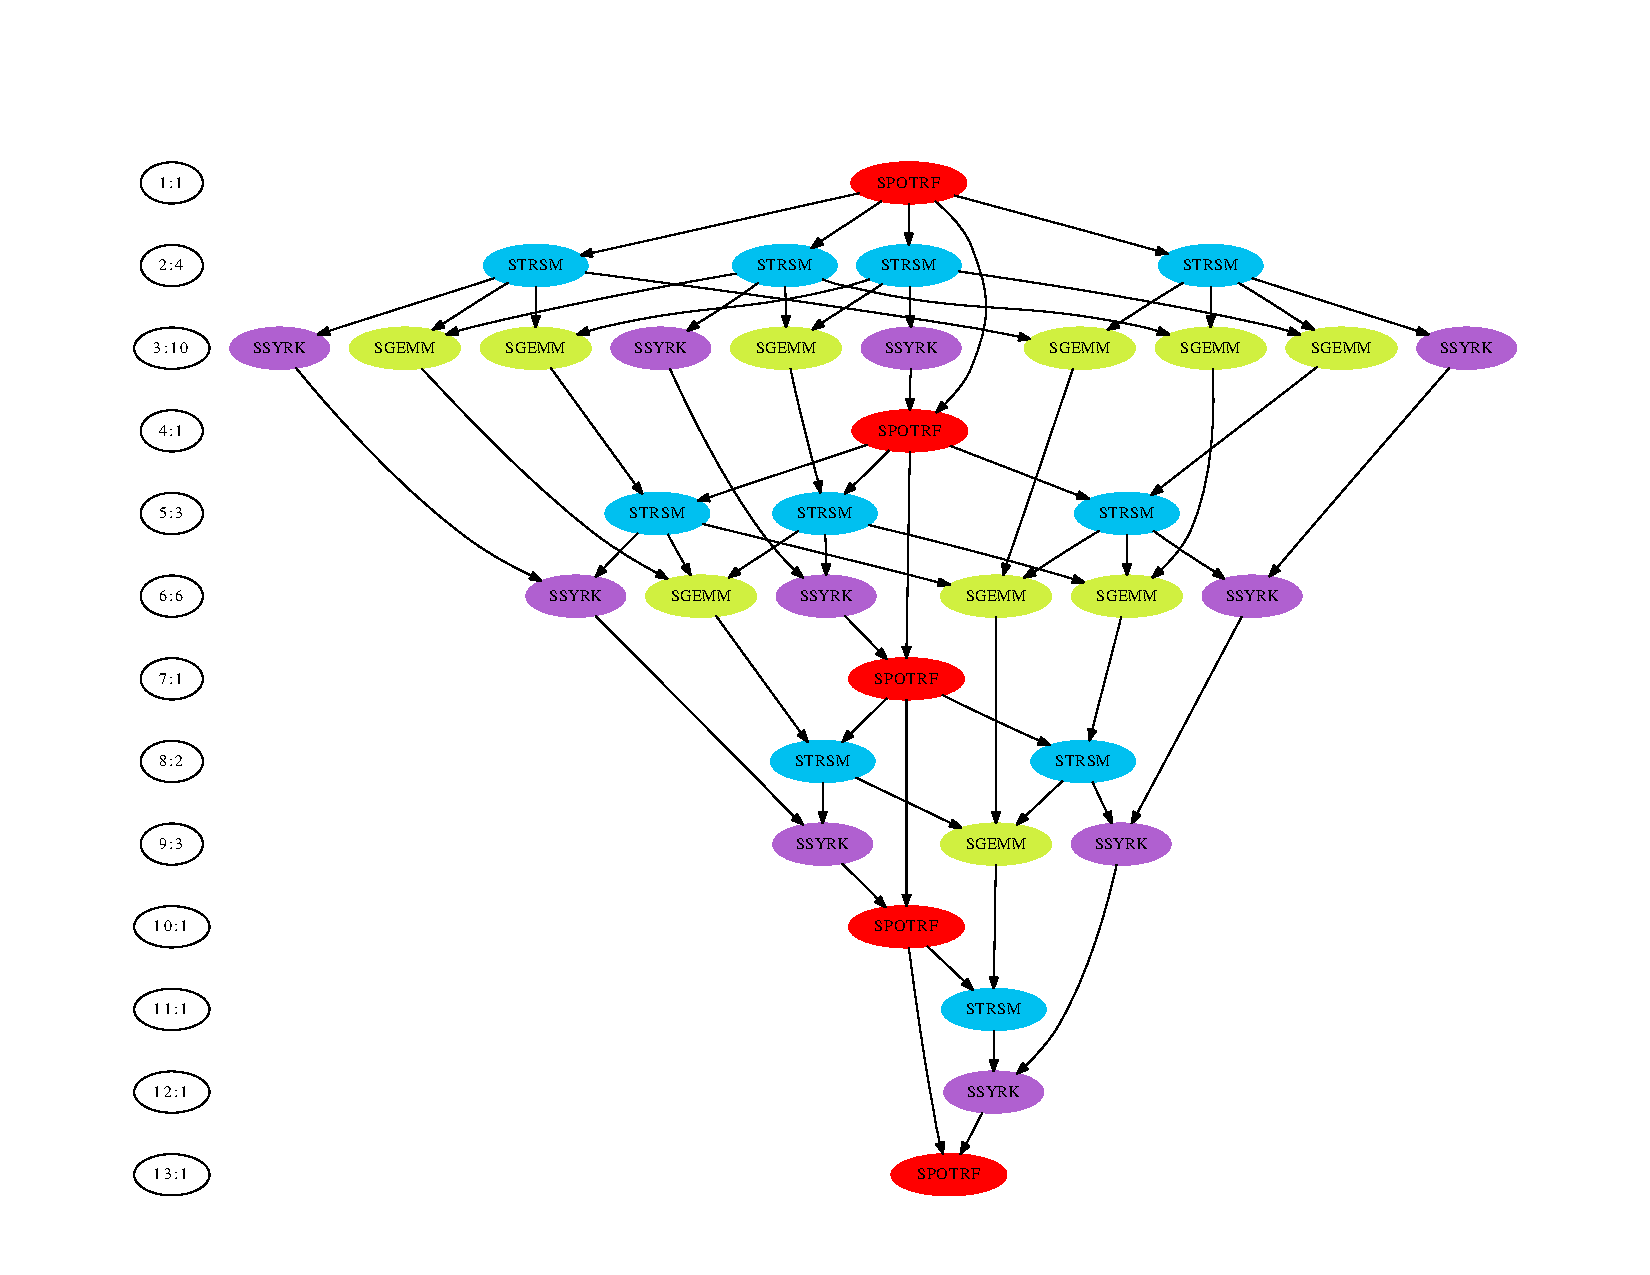
\includegraphics[width=0.9\textwidth]{dag-cholesky-5tile}
  \caption{DAG for a small Cholesky factorization (right looking
    version) with 5 tiles (block size 200 and matrix size 1000).  The
    column on the left shows the depth:width of the DAG. }
  \label{fig:DAG-Cholesky-5}
\end{figure}

The code segment shown in Fig.~\ref{fig:tileCholeskyCode} shows how
the pseudocode for Cholesky factorization in
Fig.~\ref{fig:tileCholesky} can be translated into C code.  Because
the data dependency DAG is inferred during runtime, the actual C code
looks very similar to the pseudocode.  Each of the \verb|QUARK_CORE_|
routines is a wrapper routine that inserts a task into the QUARK
runtime, adding to the paramters their size, usage (e.g. \verb|INOUT|)
and any other flags. In this example, the matrix multiplication
\verb|DGEMM| task is shown in more detail in
Fig.~\ref{fig:quark_core_dgemm}.  The use of these \verb|QUARK_CORE_|
wrapper routines makes the top level algorithm in
Fig.~\ref{fig:tileCholesky} easier to write and understand.  Each task
insertion specfies the function that is to be called when the task is
executed.  This function will unpack parameters from QUARK, and
perform the actual computation work.  The other routines are not shown
here, but can be found in the open source PLASMA linear algebra
library.
\begin{figure}[pbt]
\centering
\scriptsize
\begin{lstlisting}
    Quark *quark = QUARK_New( 0 );
    for (k = 0; k < M; k++) {
        QUARK_CORE_dpotrf( quark, &task_flags, ... );
        for (m = k+1; m < M; m++)
            QUARK_CORE_dtrsm( quark, &task_flags, ... );
        for (m = k+1; m < M; m++) {
            QUARK_CORE_dsyrk( quark, &task_flags, ... );
            for (n = k+1; n < m; n++)
                QUARK_CORE_dgemm( quark, &task_flags, ... );
        }
    }
    QUARK_Delete( quark );
\end{lstlisting}
\caption{Code outline for tiled Cholesky factorization that inserts
  the scheduled core linear algebra operations.  This is very similar
  to the pseudocode from Fig.~\ref{fig:tileCholesky}.  For simplicity,
  the arguments are not shown, however the detailed implementation can
  be found in the PLASMA library. }
\label{fig:tileCholeskyCode}
\end{figure}

\begin{figure}[pbt]
\centering
\scriptsize
\begin{lstlisting}
    void QUARK_CORE_dgemm(Quark *quark, Quark_Task_Flags *task_flags,
                      int transA, int transB,
                      int m, int n, int k, int nb,
                      double alpha, double *A, int lda,
                      double *B, int ldb,
                      double beta, double *C, int ldc)
    {
        QUARK_Insert_Task(quark, CORE_dgemm_quark, task_flags,
            sizeof(PLASMA_enum),    &transA,    VALUE,
            sizeof(PLASMA_enum),    &transB,    VALUE,
            sizeof(int),            &m,         VALUE,
            sizeof(int),            &n,         VALUE,
            sizeof(int),            &k,         VALUE,
            sizeof(double),         &alpha,     VALUE,
            sizeof(double)*nb*nb,   A,          INPUT,
            sizeof(int),            &lda,       VALUE,
            sizeof(double)*nb*nb,   B,          INPUT,
            sizeof(int),            &ldb,       VALUE,
            sizeof(double),         &beta,      VALUE,
            sizeof(double)*nb*nb,   C,          INOUT,
            sizeof(int),            &ldc,       VALUE,
            0);
    }

    void CORE_dgemm_quark(Quark *quark)
    {
        int transA; int transB; int m; int n; int k; double alpha; double *A;
        int lda; double *B; int ldb; double beta; double *C; int ldc;

        quark_unpack_args_13(quark, transA, transB, m, n, k,
            alpha, A, lda, B, ldb, beta, C, ldc);
        cblas_dgemm( CblasColMajor, transA, transB, m, n, k,
            (alpha), A, lda, B, ldb, (beta), C, ldc);
    }
\end{lstlisting}
\caption{ Implementation of the {\texttt DGEMM} kernel used in
  Cholesky factorization in the PLASMA library.  This shows the
  routine that inserts the task into the runtime, and the routine that
  unpacks the arguments and calls the {\texttt BLAS DGEMM} routine. }
\label{fig:quark_core_dgemm}
\end{figure}



%%%%%%%%%%%%%%%%%%%%%%%%%%%%%%%%%%%%%%%%%%%%%%%%%%%


\bibliographystyle{unsrt}
\bibliography{quark_users_guide}

%%%%%%%%%%%%%%%%%%%%%%%%%%%%%%%%%%%%%%%%%%%%%%%%%%%

\end{document}

%%%%%%%%%%%%%%%%%%%%%%%%%%%%%%%%%%%%%%%%%%%%%%%%%%%
